\documentclass[../../main.tex]{subfiles}

% 

\begin{document}
\chapter{Štruktúra hadrónov}

\section{Zadanie}
Kvarkový model: štruktúra baryónov a mezónov, Ťažké kvarky: podivné, pôvabné a krásne častice a top kvark, ich vlastnosti a objavy, Experimenty ukazujúce na kompozitnú štruktúru atómového jadra a nukleónov, Rutherfordov rozptyl, nepružný rozptyl, formfaktor, Rosenbluthová formula, hlboký nepružný rozptyl, partónový model, jety 

\section{Kvarkový model}
\subsection{Stručná história}
Rozvoj klasifikačných schém pre hadróny sa stal dôležitou otázkou po tom, čo nové experimentálne techniky odkryli, že veľké množstvo hadrónov nie je  elementárnych. Ukázalo sa totiž, že tieto hadróny sú viazané stavy menších komponent. Niekoľko skorých návrhov, ako napríklad Fermi-Yangov model (1949) alebo Sakatov model (1956), uspokojivo popísali mezóny avšak, zlyhali pri popise baryónov.

Gell-Mann–Nishijima formula viedla ku klasifikácii zvanej osemnásobná cesta (eightfold way), ktorú Gell-Mann vytvoril s významnými príspevkami z Ne'emanovho modelu v roku 1961. V tejto klasifikácii boli hadróny usporiadané do SU(3) reprezentatívnych multipletov: oktetov a dekupletov. Hadróny nachádzajúce sa v rovnakom multiplete mali zhruba rovnakú hmotnosť kvôli silnej interakcii. Malé hmotnostné rozdiely v týchto multipletoch boli spojené s kvantovými číslami chuti, ktoré nie sú viditeľné pre silné interakcie. Avšak, Gell-Mann-Okubo hmotnostný vzorec systematizoval kvantifikáciu týchto malých hmotnostných rozdielov medzi členmi hadrónového multipletu.

Baryón $\Omega^{-}$ so spinom 3/2, ktorý je súčasťou základného baryónového dekupletu bol rozhodujúcou predpoveďou tejto klasifikácie. Gell-Mann pomocou tejto klasifikácie predpovedal túto časticu v roku 1962. V roku 1964 v BNL bola pozorovaná častica, ktorá mala požadované vlastnosti ako častica $\Omega^{-}$.

V roku 1964, ešte pred objavením $\Omega^{-}$ častice, Gell-Mann a George Zweig publikovali nezávisle na sebe články, v ktorom vysvetlili čo je zakódované v eightfold way klasifikácii. V tomto článku postulovali elementárne fermiónové komponenty, ktoré nie je možné pozorovať voľne v prírode - kvarky. Rozdiely v hmote hadrónov boli teraz spojené s rôznymi hmotnosťami kvarkov. Tento model bol nazvaný kvarkový model. Gell-Mann a Zweig navrhli, že usporiadanie hadrónov do mutlipletov je možné vysvetliť, pokiaľ hadróny budú tvorené kvarkmi:
\begin{itemize}
\item mezóny ($q\bar{q}$): $3\otimes \bar{3}=1\oplus 8$
\item baryóny ($qqq$): $3 \otimes 3 \otimes 3 = 1 \oplus 8 \oplus 8 \oplus 10$  
\end{itemize}

\subsection{Kvarkový model}
Kvarkový model je klasifikačná schéma pre hadróny z hľadiska ich valenčných kvarkov, ktoré udávajú kvantové čísla hadrónov. Kvarkový model vychádza z flavour SU(3), úspešnej klasifikačnej schémy organizujúcej veľký počet ľahších hadrónov, ktoré boli objavené 50. až 60. rokoch minulého storočia a je platnou účinnou klasifikáciou doteraz. Tento model navrhli v roku 1964 nezávisle na sebe dvaja páni, Murray Gell-Mann a George Zweig. V súčasnej dobe bol model v absorbovaný ako súčasť zavedenej kvantovej teórie poľa silných a elektroslabých interakcií, zvanej Štandardný model. Eightfold way organizuje mezóny a baryóny so spinom 1/2 do oktetu, princípy eightfold way sa dajú aplikovať aj na baryóny so spinom 3/2, ktoré tvoria dekuplet.

Ako sme už spomínali, hadróny nie sú elementárne a považujú sa za viazané stavy valenčných kvarkov a antikvarkov, ktoré udávajú kvantové čísla hadrónov. Tieto kvantové čísla sú rozdelené na dva druhy. Jedna sada pochádza z Poincareho symetrie - $J^{PC}$, kde J, P a C predstavujú celkový moment hybnosti, symetriu parity a symetriu náboja. 

Zvyšné sú flavour kvantové čísla, ako je izospin, podivnosť, pôvab atď. Silná interakcia, ktorá viaže kvarky je necitlivá na tieto kvantové čísla, takže ich variácia vedie k systematickým hmotnostným a spojovacím vzťahom medzi hadrónmi v rovnakom aromatickom multiplete.

\begin{itemize}
\item flavour: u, d, s, c, b, t - kvarky + príslušné antikvarky
\item náboj (Q): Q = -1/3 pre (d, s, b), Q = 2/3 pre (u, c, t)
\item baryónové číslo (B): B = 1/3 pre kvarky, B = -1/3 pre antikvarky
\item strangenss (S): $S_s$ = -1, $S_{\bar{s}}$ = 1, $S_{u,d,c,t,b}$ = 0
\item charm (C): $C_c$ = 1, $C_{\bar{c}}$ = -1, $C_{u,d,s,t,b}$ = 0
\item bottomness ($B^{\prime}$): $B^{\prime}_b$ = -1, $B^{\prime}_{\bar{b}}$ = 1, $B^{\prime}_{u,d,s,t,c}$ = 0
\item topness (T): $T_t$ = 1, $T_{\bar{t}}$ = -1, $T_{u,d,s,c,b}$ = 0
\item izospin (I): I = 1/2 pre (u, d), I = 0 pre (s, c, t, b)
\item 3. zložka izospinu ($I_3$): $I_3$ = 1/2 pre u, $I_3$ = -1/2 pre d, $I_3$ = 0 pre (s, c, t, b),
\end{itemize}
Kvarky sú častice so spinom 1/2 a preto sú to fermióny. Každý kvark a antikvark podlieha Gell-Mann-Nishijima formule
\begin{equation}
Q=I_3+\frac{Y}{2}=I_3+\frac{B+S+C+B^{\prime}+T}{2},
\end{equation}
kde $Y$ je hypernáboj.

Mezóny sú zložené z páru kvark-antikvark a preto majú nulové baryónové číslo, zatiaľ čo baryóny sú zložené z troch kvarkov a tak majú baryónové číslo rovné 1.

Hadróny s podobnou hmotnosťou (+spinom a paritou) ale rôznym elektrickým nábojom môžme usporiadať do izospinových multipletov, napr. (nukleónový dublet, piónový triplet). Z experimentov bolo vidieť, že podivné hadróny boli ťažšie ako nepodivné hadróny a preto sa naskytuje možnosť spojiť podivné častice s izospinovými multipletmi. 

Ďalej môžme v izospinovom priestore definovať posunovacie operátory, ktorými sme schopný prechádzať medzi jednotlivými stavmi $\pi^{+}$, $\pi^{-}$ a $\pi^{0}$. Ale čo po zavedení podivnosti? Môžme sa posúvať medzi jednotlivými mezónmi v rámci multipletu podobným spôsobom? Nato aby sme to mohli spraviť musíme zadefinovať ďalší posunovací operátor, ktorým sme schopný posúvať stavy v smere S. A preto je prirodzené rozšíriť SU(2) grupu na SU(3) grupu. Fundamentálna reprezentácia SU(3) je triplet, viď obrázok \ref{sf2:fig:triplet}. Generátory danej grupy sú Gell-Manove $3 \times 3$ matice $\lambda_i$, kde $i=1,... 8$. 

\begin{figure}[!h]
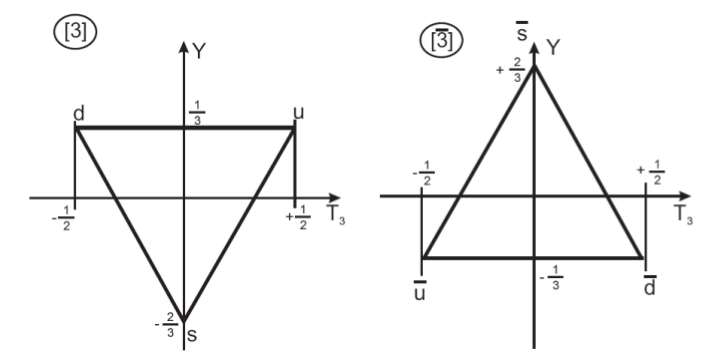
\includegraphics[width=0.7\textwidth]{subatom-02-triplet.png}
\centering
\caption{Triplet a antitriplet SU(3) grupy.}
\label{sf2:fig:triplet}
\end{figure}

SU(3) obsahuje 3 SU(2) podgrupy s príslušnými posunovacími operátormi 
\begin{itemize}
\item $T_{\pm} = F_1 \pm iF_{2}$
\item $U_{\pm} = F_6 \pm iF_{7}$
\item $V_{\pm} = F_4 \pm iF_{5}$
\item $T_3 = F_3$
\item $Y = \frac{2}{\sqrt{3}}F_8,$
\end{itemize}
kde $F_i = \frac{\lambda_i}{2}$. Akékoľvek dve podgrupy a ich príslušné posunovacie operátory sú dostatočné na zostrojenie multipletu, viď obrázok \ref{sf2:fig:operatory}. 

\begin{figure}[!h]
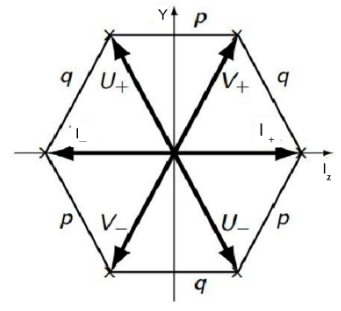
\includegraphics[width=0.4\textwidth]{subatom-02-operatory.png}
\centering
\caption{Grafické znázornenie operátorov pre jednotlivé SU(2) podgrupy grupy SU(3)}
\label{sf2:fig:operatory}
\end{figure}

Skladaním kvarkového tripletu a antitripletu môžme dostať pseudoskalárne mezóny. Grafické znázornenie daného pseudoskalárneho ($J^{PC}=0^{-+}$) multipletu je na obrázku \ref{sf2:fig:pseudoskalar}. Hmotnosť podivných mezónov je asi o $150\,\unit{MeV}$ väčšia ako hmotnosť nepodivných mozónov.

\begin{figure}[!h]
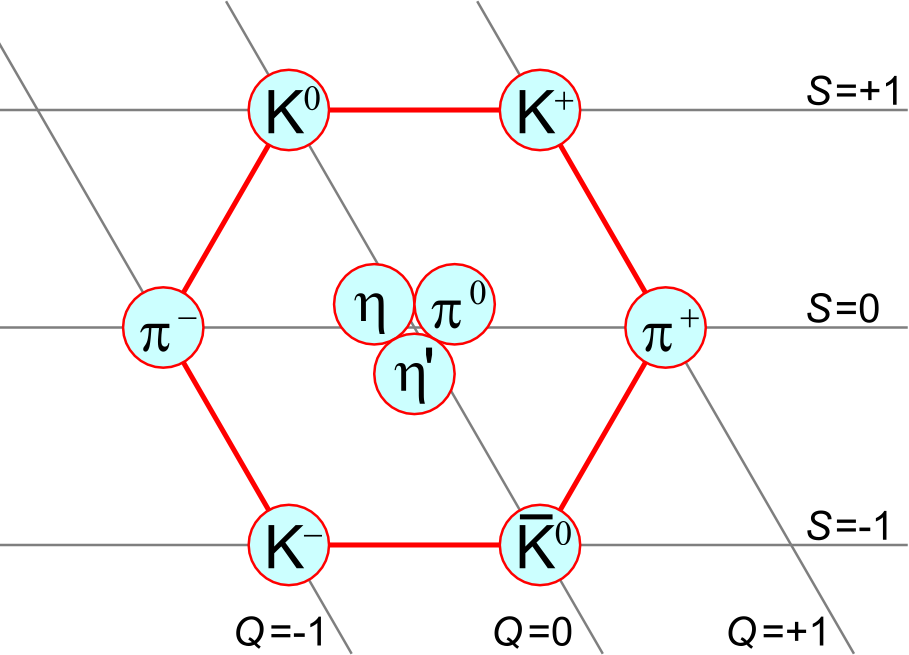
\includegraphics[width=0.5\textwidth]{subatom-02-pseudoskalar.png}
\centering
\caption{Pseudoskalárne mezóny so spinom 0.}
\label{sf2:fig:pseudoskalar}
\end{figure}

Zložením tripletu a antitripletu môžme taktiež dostať vektorové mezóny ($J^{PC}=1^{--}$). Tie sa na rozdiel od pseudoskalárnych mezónov môžu rozpadať slabou ale aj silnou interakciou, napr. $\rho^0 \rightarrow \pi^{+}\pi^{-}$ alebo $K^{*0} \rightarrow K^{+}\pi^{-}$. Grafické znázornenie vektorového multipletu je na obrázku \ref{sf2:fig:vektor}.

\begin{figure}[!h]
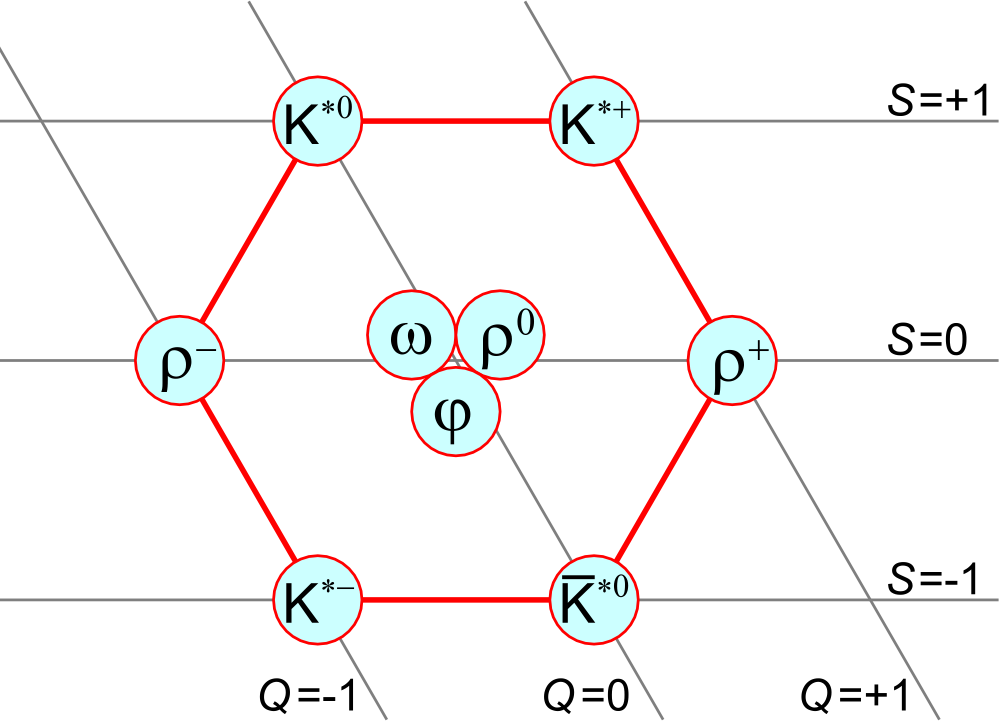
\includegraphics[width=0.5\textwidth]{subatom-02-vektor.png}
\centering
\caption{Vektorové mezóny so spinom 1.}
\label{sf2:fig:vektor}
\end{figure}

Zložením 3 tripletov môžme získať baryónový oktet ($J^P=1/2^{-}$): najľahšie baryóny rozpadajúce sa slabou interakciou okrem stabilného protónu (viď obrázok \ref{sf2:fig:baryonoctet}) alebo baryónový dekuplet ($J^P=3/2^{-}$) silne sa rozpadajúcich rezonancii (viď obrázok \ref{sf2:fig:baryondecuplet}). 

\begin{figure}[!h]
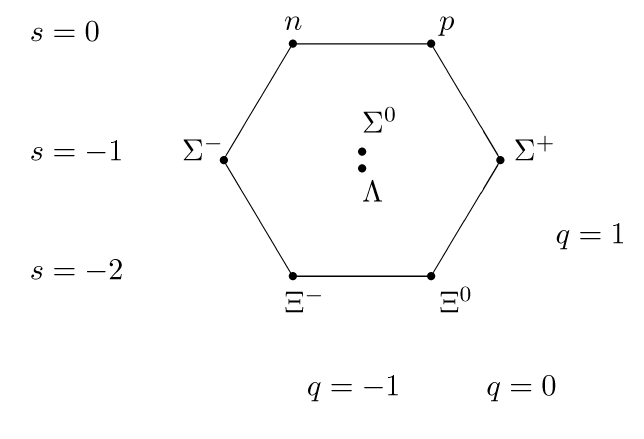
\includegraphics[width=0.6\textwidth]{subatom-02-baryonoctet.png}
\centering
\caption{Baryónový oktet pre častice so spinom 1/2.}
\label{sf2:fig:baryonoctet}
\end{figure}

\begin{figure}[!h]
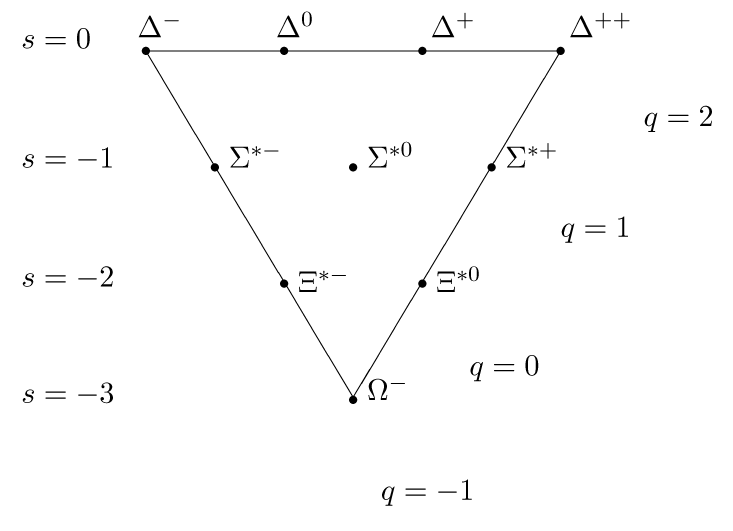
\includegraphics[width=0.6\textwidth]{subatom-02-baryondecuplet.png}
\centering
\caption{Baryónový dekuplet pre častice so spinom 3/2.}
\label{sf2:fig:baryondecuplet}
\end{figure}

\textbf{Zhrnutie vlastnosti základných $SU(3)_f$ baryónových a mezónových multipletov.}
\begin{itemize}
\item usporiadanie pozorovaných hadrónov s rovnakým spinom, paritou a baryónovým číslom do multipletov na základe ich hmotnosti a izospinovej symetrie
\item hmotnosť v izospinových multipletoch rastie s absolútnou hodnotou podivnosti
\item špeciálne jednoduchý je hmotnostný nárast v baryónovom dekuplete, 4 izospinove multiplety sú ekvidištantne separované o $\sim 150\,MeV$ 
\item silná interakcia zachováva 3. zložku izospinu a podivnosť 
\end{itemize}

Je nám známe, že kvarky sú fermióny so spinom 1/2. Pre 3 kvarky potom máme celkovo 6 stavov $\rightarrow$ naskytá sa možnosť rozšíriť SU(3) na SU(6). Potom úplná dekompozícia 3 kvarkových sextetov je:
$6 \otimes 6 \otimes 6 = 56 \oplus 70 \oplus 70 \oplus 20 $. Pre mezóny dostávame $6 \otimes \bar{6} = 35 \oplus 1$. Všetky baryóny 56-tipletov musia mať plne symetrické vlnové funkcie voči permutáciám konštituentných kvarkov.\newline

\textbf{Magnetické momenty baryónov}\newline
Baryón je zložený z kvarkov, ktoré uvažujeme ako bodové fermióny: 
\begin{equation}
\mu_B = \sum_{q=u,d,s} \mu_q = \sum_{q=u,d,s} \langle B,\uparrow \vert \mu_3^q  \vert B,\uparrow \rangle,
\end{equation}
kde $\mu_3^q= e_q\sigma_3/2m_q $. Uveďme si nejaký príklad magnetického momentu, ktorý sa spočíta pomocou kvarkového modelu:
\begin{itemize}
\item protón: $\mu_p = (4\mu_u - \mu_d)/3$
\item neutrón: $\mu_n = (4\mu_d - \mu_u)/3$
\item $\Lambda$: $\mu_{\Lambda} = \mu_s$
\end{itemize}
Použitím experimentálne určených magnetických momentov protónu (2.793), neutrónu (-1.913) a lambda mezónu (-0.613) sme schopný dostať magnetické momenty jednotlivých kvarkov: $\mu_u = 1.852$, $\mu_d = -0.972$, $\mu_s = -0.613$.\newline

\textbf{Okubo-Zweig-Iizuka (OZI) pravidlo}\newline
V 60. rokoch 20. storočia bolo namerané, že sa $\phi$ mezón rozpadá silnou interakciou na kaóny viac než sa očakávalo
\begin{itemize}
\item $BR(\phi \rightarrow K^+K^-) = 48.9 \pm 0.5 \%$
\item $BR(\phi \rightarrow K_LK_S) = 34.2 \pm 0.4 \%$
\item $BR(\phi \rightarrow \rho \pi+\pi^+ \pi^- \pi^0) = 15.32 \pm 0.32 \%$
\end{itemize}
aj napriek tomu, že rozpad na pióny bol kinematický výhodnejší než na kaóny
\begin{itemize}
\item $\Delta m(\phi \rightarrow \pi^{+} \pi^{-} \pi^{0})= (1020-415) = 605\,MeV/c^{2}$
\item $\Delta m(\phi \rightarrow \rho^{+} \pi^{-})= (1020-909) = 111\,MeV/c^2$
\item $\Delta m(\phi \rightarrow K^{+} K^{-})= (1020-988) = 32\,MeV/c^2$
\end{itemize}
Páni Okubo, Zweig a Iizuka nezávisle na sebe navrhli fenomenologické pravidlo vysvetľujúce účinné prierezy a pravdepodobnosti rozpadu v rámci aditívneho kvarkového modelu: \textbf{Koncový stav procesov riadených silnou interakciou, ktorý môže byť dosiahnutý len anihiláciou kvarku a antikvarku je potlačený alebo inak, ak je možné diagram rozdeliť odstránením gluónových/fotónových čiar na aspoň dve časti, potom je tento fyzikálny kanál potlačený.}
Základnú myšlienku tohto pravidla môžme znázorniť pomocou tzv. kvar-flow diagramov, ktoré popisujú tok kvarkov danej vône z počiatočného do koncového stavu. Tieto diagramy môžme rozdeliť na dve skupiny:
\begin{itemize}
\item povolené: planárne diagramy sú spojené tj. diagram sa nedá rozdeliť na 2 časti bez toho aby sme prerušili kvarkovú líniu
\item zakázané: planárne diagramy môžme rozdeliť na dve časti bez toho aby sme prerušili kvarkovú líniu
\end{itemize}

\begin{figure}[!h]
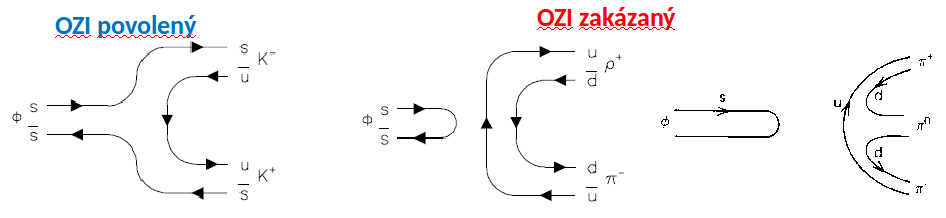
\includegraphics[width=1.0\textwidth]{subatom-02-OZI.png}
\centering
\caption{Povolené a zakázané kanály určené pomocou OZI pravidla.}
\label{sf2:fig:OZI}
\end{figure}

Zakázané procesy sú potlačené voči tým povoleným avšak, miera potlačenia nie je jednoznačne určená. Takže v našom príklade na obrázku (\ref{sf2:fig:OZI}) rozpad $\phi \rightarrow \pi^{-} \rho^{+}$ je potlačený voči $\phi \rightarrow K^{+} K^{-}$.\newline

\textbf{Problémy aditívneho kvarkového modelu}
\begin{itemize}
\item kvarky nie sú v prírode pozorované voľne a neexistuje žiadna indikácia pre existenciu exotických stavov ako napríklad sextet symetrických kombinácii dikvarku.
\item neboli pozorované stavy: $2q2\bar{q}$ a $4q\bar{q}$, ktoré sú povolenými kombináciami $q\bar{q}$ a $3q$. 
\end{itemize}
Predpoklad, že kvarky nie sú fermióny, ale tzv. parafermióny ranku 3. Toto vyriešilo problém so štatistikou, pretože v každom stave mohli byť maximálne 3 parafermióny. Veľmi skoro sa ukázalo, že idea paraštatistiky je ekvivalentná predpokladu, že každá kvarková vôňa (flavor) existuje v 3 farebných stavoch a pozorované hadróny odpovedajú bezfarebným stavom. V jazyku teórie grúp to znamená, že kvarky sa transformujú ako fundamentálny triplet novej SU(3) grupy, tzv. Color SU(3) označovanej ako $SU(3)_C$. Pozorované hadróny sú postulované ako farebné singlety:
$$ \vert baryon^{\alpha \beta, \gamma} \rangle = \epsilon^{ijk} \vert q_i^{\alpha} \rangle \vert q_j^{\beta} \rangle \vert q_k^{\gamma} \rangle,$$
kde i,j,k sú farebné indexy a $\alpha, \beta, \gamma$ sú vône kvarku.

Dôsledky zavedenia farebného náboja sú, že k vytvoreniu farebného singletu je potrebné aspoň toľko farieb, aký je počet kvarkov v baryóne, tj. nie je možné pozorovať dikvark, ale stále to ešte nevylučuje existenciu $4q\bar{q}$ stavu. Pre mozóny nie je žiadne obmedzenie, pretože pre akýkoľvek počet farieb priamy produkt fundamentálnej reprezentácie a jej komplexne združenej reprezentácie obsahuje singlet. Problém sa vlastne preformuloval na otázku: prečo existujú v prírode len farebné singlety? 

Dôležitý posun vpred prišiel v roku 1965 v tzv. Nambu modely. Uväznenie kvarkov je dôsledkom supersilnej interakcie medzi fundamentálnymi objektmi, kde supersilná interakcia pôsobiaca medzi kvarkmi je sprostredkovaná oktetom kalibračných polí $G_{\mu}$, $\mu = 1 ... 8$ viazaných do infinitezimálnych SU(3) generátorov $\lambda_{\mu}$.\newline

\textbf{Nambu model}
\begin{itemize}
\item základ dnešného QCD, 8 rokov pred formuláciou QCD ako kvantovej teórie poľa
\item interakcia medzi kvarkmi je sprostredkovaná výmenou oktetov farebných kalibračných bozónov a má nasledujúce vlastnosti:
\begin{enumerate}
\item kvarky ako individuálne častice sú nekonečne ťažké tj. nepozorovateľné
\item sila medzi kvarkmi je príťažlivá vo farebných singletoch, tj. viazané stavy s konečnou hmotnosťou
\item vo všetkých ďalších kanáloch je interakcia odpudivá, tj. systém je nekonečne ťažký a nepozorovateľný 
\item sila $F(q\bar{q})$ v mezónoch je 2x väčšia než $F(qq)$ 
\end{enumerate}
\item farebný potenciál je rozšírením typickej spin-spin interakcie
$$ V_{ij} = \frac{1}{8} \sum_{i \neq j}^{n} v(\vec{r}_{ij}) \vec{\lambda_{i}}\vec{\lambda_{j}} $$
\end{itemize}

\subsection{Ťažké kvarky (s,c,t,b)}
\textbf{S kvark - vlastnosti a objavenie}
\begin{itemize}
\item holá (bare) hmotnosť: $95\,\unit{MeV}/c^2$, spin: $1/2$, náboj: $-\frac{1}{3}e$ 
\item nachádza sa napríklad v kaónoch, podivných D mezónoch, $\Sigma$ baryónoch ...
\end{itemize}

Pravdepodobne prvá podivná častica ($m=500\pm 6 \,MeV$ asi $K^{+}$) bola pozorovaná už v roku 1943 v hmlovej komore v Pyrenejach. Avšak skutočná éra objavov podivných častíc nastala v roku 1947. V tomto roku boli pozorované dve nové častice v hmlových komorách:
\begin{itemize}
\item $V^{0}$ častica: neutrálna častica, ktorá sa rozpadá na pár opačne nabitých častíc, jej hmotnosť bola $m=440\pm 100 \,MeV$ asi $K^{0}$
\item rozpad kladne nabitej častice s $m=540\pm 100 \,MeV$ asi $K^{+}$
\end{itemize}
V rokoch 1950-1952 experimenty ukázali existenciu dvoch $V^{0}$ častíc:
\begin{itemize}
\item $V^{0}_1$ rozpad častice na $\pi^{+}\pi^{-}$, $m \sim 500 \,MeV$ asi $K^{0}$
\item $V^{0}_2$ rozpad na protón a $\pi^{-}$, $m \sim 1100 \,MeV$ asi $\Lambda$
\end{itemize}
Pri pozorovaní týchto častíc bolo zrejmé, že tieto častice sa správajú podivne (pomenovanie zaviedol Gell-Mann) tj. rozpadajú sa o mnoho rádov pomalšie ($10^{-10}$) než silné rozpady ($10^{-23}$). V roku 1953 Gell-Mann navrhol priradiť izospin novým podivným časticiam, aby zdôvodnil prečo sa nerozpadajú silnou interakciou.

Experimenty v BNL ukázali dôležitú vlastnosť produkcie podivných častíc, tzv. asociatívnu produkciu: podivné častice sú produkované v pároch s opačnou podivnosťou, čo je dôsledkom zachovania podivnosti v silnej interakcii.

V roku 1954 Nishijima reformuloval priradenie izospinu časticiam pomocou nového kvantového čísla $\nu$ náboj. Neskôr sa pre tento náboj ujalo Gell-Mannovo pomenovanie - podivnosť (strangeness). Podivnosť sa zachováva v silnej interakcii ale nezachováva sa v slabej interakcii. Zaviedla sa Gell-Mann-Nishijimová formula
$$ Q = T_3 + \frac{B+S}{2} = T_3 + \frac{Y}{2},$$
V SU(3) je zachovanie izospinu ekvivalentné zachovaniu podivnosti. Takže táto formula neprináša žiadne obmedzenie na možné silné rozpady. Viacmenej zavedenie podivnosti bolo kľúčové pretože to otvorilo cestu unitárnej symetrii a kvarkovému modelu. 
Na konferencii v Pise v roku 1954 Gell-Mann predpovedal existenciu $\Xi^0$ (objav 1956) a $\Sigma^0$ (objav 1959) a v apendixe pripojil aj predpoveď existencie baryónu $\Omega^-$ (objav 1964).

V roku 1952-1954 Fermi, pozoroval prvú rezonanciu: $\Delta^0$, pík v $\sigma(\pi^{-}p \rightarrow \pi^{-}p)$. V 1955 na Cosmotrone v BNL bola potvrdená existencia tejto Fermiho rezonancie a navyše sa ukázalo, že existuje vo všetkých $\pi N$ kanáloch a má teda spin 3/2. 

V roku 1961 na Bevatrone, na $\pi^{-}p$ zrážkach, bol objavený prvý vektorový mezón: $K^{*-}$ Potom nasledovali objavy ďalších rezonancií: $\rho$, $\omega$, $\phi$... V roku 1962 v Ženeve, oznámenie objavov baryónových rezonancii $\Xi^{*}$ a $\Xi^{*0}$. 

Napriek veľkému množstvu objavených podivných častíc, existencia samotného podivného kvarku bola postulovaná až v roku 1964 Gell-Mannon a Zweigom, aby bolo možné vysvetliť klasifikačnú schému hadrónov známu ako osemnásobná cesta. Prvé experimentálne náznaky existencie tohto kvarku prišli v roku 1968 v hlboko neelastických rozptylových experimentoch na SLAC-u. Na tomto zariadení sa potvrdila aj existencia kvarkov u, d.
\newline

\textbf{C kvark - vlastnosti a objavenie}
\begin{itemize}
\item holá (bare) hmotnosť: $1.29\,\unit{GeV}/c^2$, spin: $1/2$, náboj: $\frac{2}{3}e$ 
\item nachádza sa napríklad v $J/\Psi$ mozóne, D mezónoch, charmed Sigma baryón $\Sigma_c$...
\item $J/\Psi$ sa rozpadá 1000x pomalšie ako napríklad $\rho$, 
\end{itemize}

Krátko po formulácii kvarkového modelu s u, d, s kvarkmi, sa začalo špekulovať o existencii 4. kvarku, ktorý bol pomenovaný Bjorkenom a Glashowom ako charm kvark. Prečo by ale mal tento kvark existovať?
\begin{enumerate}
\item symetria medzi kvarkmi a leptónmi (3 kvarky 4 leptóny) - v roku 1962 objavenie $\nu_{\mu}$ neutrína.
\item oveľa akútnejšie bolo potrebné vyriešiť 2 závažné problémy v teórii slabých interakcii
\begin{itemize}
\item silné potlačenie Flavor changing neutral currents procesov:
$$ K_L \rightarrow \mu^+ \mu^- \hspace{1cm} BR = 7.2\times 10^{-9} $$
$$ K^+ \rightarrow \pi^+ e^+ e^- \hspace{1cm} BR = 2.7\times 10^{-7} $$
\item axiálne anomálie
\end{itemize}
\end{enumerate}
Tieto problémy sa automaticky vyriešia zavedením 4. kvarku s nábojom 2/3 a spinom $ 1/2$. Jeho hmotnosť však musí byť $ m_c \leq 2\,GeV/c^2 $.

Aj napriek špekuláciám, ktoré mali Bjorken a Glashow, sa predpoveď c kvarku pripisuje pánom Glashow, Iliopoulos a Maioni v roku 1970. Prvou pozorovanou časticou, ktorá obsahuje c kvark bola častica $J/\Psi$ mezón. Tá bola objavená na dvoch zariadeniach v roku 1974. Prvé zariadenie bol urýchľovač SPEAR na SLAC-u. Tím vedený pánom Richterom pozoroval nárast účinného prierezu v zrážkach $e^+e^-$. Táto častica bola nazvaná $\Psi$. Na druhej strane Ameriky v BNL sa tím vedený pánom Tingom venoval hľadaniu ťažkých fotónov. Používal sa nato výborný detektor: magnetický spektrometer s 2 ramenami + Čerenkovovskými detektormi na identifikáciu elektrónov a pozitrónov v reakcii ($p+Be \rightarrow e^+e^- + $niečo). V BNL začali poriadne prehľadávať oblasť medzi $3-5\,GeV/c^2$ v $m_{ee}$ a nakoniec pozorovali jasný signál pri $m_{ee}=3.1\,GeV/c^2$. Túto časticu nazvali $J$. V priebehu 10 dní, od oznámenia $J/\Psi$ mezónu, tím na experiment SPEAR pozoroval ďalší vektorový mezón $\Psi^{\prime}$, čo bol v podstate excitovaný stav $J/\Psi$.

Spektrum charmonií sa dá dobre teoretický popísať v rámci nerelativistickej kvantovej mechaniky pomocou potenciálu 
$$ V(r)=-\frac{4\alpha_s}{3r}+kr,$$ 
kde $\alpha_s$ je väzbová konštanta a k je strunové napätie zodpovedajúce uväzneniu.

Hadrónový rozpadový mód $J/\Psi$ častice je silno potlačený pretože D mezóny sú príliš ťažké a rozpad na pár D mezónov nemôže ísť cez OZI povolený diagram ale len cez OZI zakázaný diagram, viď obrázok (\ref{sf2:fig:OZIJPSI}). Tento fakt výrazne zvyšuje životnosť častice a tým je rozpadová šírka častice veľmi malá, $93,2\,\unit{keV}$. Kvôli tomuto silnému potlačeniu elektromagnetické procesy začnú konkurovať hadrónovým rozpadom. To je dôvod prečo má $J/\Psi$ taký významný Branching ratio pre leptóny. Open charm mezóny (D, $D^*$, $D_s,...$) sú viazané stavy c alebo ($\bar{c}$) s (u, d, s) kvarkmi. Tieto mezóny boli objavené v roku 1976.

Takže zopakujem dôležitú časť. Z časti, kde sme preberali OZI pravidlo vieme, že procesy, v ktorých dochádza k anihilácií sú silno potlačené. To by znamenalo, že v rozpade $J/\Psi$ mezónu bude dominovať rozpad na D mezóny. Avšak tento rozpad nie je kinematický možný, keďže dva najľahšie D mezóny majú dokopy viacej ako ma $J/\Psi$. Preto je tento mezón o niečo viacej stabilnejší, čo spôsobí to, že jeho rozpadová šírka je dosť malá a hadrónovým rozpadom začnú konkurovať tie elektromagnetické.

\begin{figure}[!h]
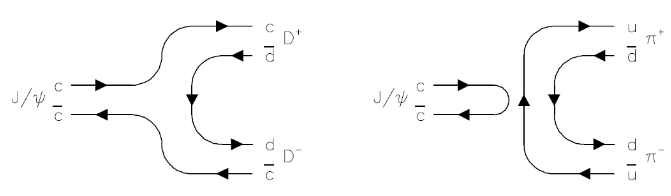
\includegraphics[width=0.9\textwidth]{subatom-02-OZIJPSI.png}
\centering
\caption{Diagramy pre rozpad charmónia na pár mezónov obsahujúcich charm kvark (vľavo) alebo diagram rozpadu charmónia na mezóny, ktoré neobsahujú charm kvark (vpravo). V tomto diagrame dochádza k anihilácii $c \bar{c}$.}
\label{sf2:fig:OZIJPSI}
\end{figure}

Objavom c kvarku je tak SU(3) symetria povýšená na SU(4). Medzi SU(3) a SU(4) existujú podstatné rozdiely napr. existujú 3 vzájomné komutujúce generátory: $T_3$, Y, C, kde C odpovedá zachovávajúcemu sa charm kvantovému číslu. Gell-Mann-Nishijimova formula preto dosiahne tvar 
$$ Q = T_3 + \frac{B+S+C}{2} = T_3 + \frac{Y+C}{2}.$$
A aj multiplety sa nám trochu pozmenia, viď obrázok (\ref{sf2:fig:multiplets}).

\begin{figure}[!h]
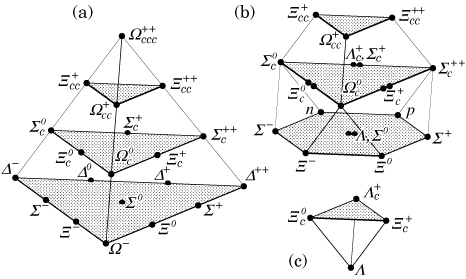
\includegraphics[width=0.9\textwidth]{subatom-02-multiplets.jpg}
\centering
\caption{Multiplety po zavedení c kvarku.}
\label{sf2:fig:multiplets}
\end{figure}


\textbf{b kvark - vlastnosti a objavenie}
\begin{itemize}
\item holá (bare) hmotnosť: $4.65\,\unit{GeV}/c^2$, spin: $1/2$, náboj: $-\frac{1}{3}e$ 
\item nachádza sa napríklad v Upsilon mezóne ($\Upsilon$) s $m \approx 9.41\,\unit{GeV}/c^2$, ($\Upsilon^{\prime}$) s $m \approx 10.06\,\unit{GeV}/c^2$, ($\Upsilon^{\prime \prime}$) s $m \approx 10.44\,\unit{GeV}/c^2$
\end{itemize}

Situácia po objavení c kvarku: dve úplné generácie kvarkov a leptónov. Ale už v roku 1975 bol na SLAC-u objavený leptón tau - tretia generácia leptónov. Automaticky sa naskytla otázka, či existuje aj ďalší kvark. Predpokladané tau neutríno bolo objavené v roku 2000. Teoretický bol b kvark navrhnutý Maskawom a Kobayashim. Kvark b bol objavený v roku 1977 vo Fermilabe tímom, ktorý viedol pán Lederman, pri produkcii bottomónia ($b \bar{b}$).\newline

\textbf{t kvark - vlastnosti a objavenie}
\begin{itemize}
\item holá (bare) hmotnosť: $172.44\,\unit{GeV}/c^2$, spin: $1/2$, náboj: $\frac{2}{3}e$ 
\end{itemize}

Kvark t interaguje primárne silnou interakciou ale rozpadá sa iba slabou interakciou. Rozpadá sa na W bozón a b kvark (najčastejšie), s kvark alebo d kvark (najmenej), viď obrázok \ref{sf2:fig:t}. Podľa štandardného modelu jeho stredná doba života je zhruba $5\cdot 10^{-25}\,\unit{s}$ a preto netvorí hadróny. Jeho existenciu predpovedali Maskawa a Kobayashi v roku 1973 spoločne s b kvarkom aby vysvetlili CP narušenie v kaónovom rozpade. Kvark t bol objavený v roku 1995 na experimentoch CDF a D0 vo Fermilabe. Spoločne s b kvarkom tvorí tretiu generáciu kvarkov.

\begin{figure}[!h]
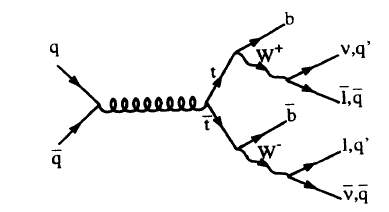
\includegraphics[width=0.5\textwidth]{subatom-02-t.png}
\centering
\caption{Schéma rozpadu t kvarku.}
\label{sf2:fig:t}
\end{figure}

\subsection{Experimenty ukazujúce na kompozitní štruktúru atómového jadra a nukleónov}

Na začiatku 20. storočia sa predpokladalo, že kladný náboj je v atóme rozdelený rovnomerne a elektróny sa vyskytujú v celom objeme atómu, tzv. pudingov model atómu. Experiment založený na rozptyle alfa častíc na jadrách zlata to mal potvrdiť. Na veľké prekvapenie to však vyvrátil. Ukázalo sa totiž, že dochádza k rozptylu na potenciáli $V(r)=const/r$. Účinný prierez mal nasledujúci tvar
$$ \frac{d\sigma}{d\Omega} = \frac{\alpha^2}{16 E^2 sin^4(\theta/2)} = \frac{4\alpha^2m^2}{q^4},$$
kde $q$ je prenesená hybnosť, $\theta$ je uhol rozptylu a $m$ je hmotnosť častice. Dáta z tohto experimentu sú znázornené na obrázku \ref{sf2:fig:rutherford}.

\begin{figure}[!h]
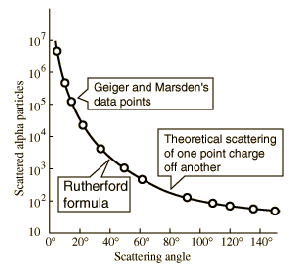
\includegraphics[width=0.5\textwidth]{subatom-02-rutherford.png}
\centering
\caption{Dáta z Rutherfordovho experimentu, ktoré vyvrátili pudingov model atómu.}
\label{sf2:fig:rutherford}
\end{figure}

Štúdium atómového jadra začalo štúdiom elastického rozptylu. S odstupom času sa dokázali zrážať jadra pri väčších energiách, čo umožňovalo hlbšie skúmanie štruktúry jadra a nukleónov a prechod od elastických k neelastickým rozptylom. Skôr než začneme s jednotlivými experimentmi, zavedieme si potrebnú kinematiku rozptylu.

Na začiatok si zavedieme Lorentzovsky invariantné veličiny
\begin{itemize}
\item $x=\frac{Q^2}{2p_2q}$ kde $Q^2=-q^2>0$, elasticky rozptyl: $x=1$, neelastický rozptyl $0<x<1$
\item $y=\frac{p_2q}{p_2p_1}$, kde $0<y<1$ - časť stratenej energie prichádzajúcej častice, v lab. $y=1-\frac{E_3}{E_1}$
\item $\nu = \frac{p_2q}{M}$ - energia stratená prichádzajúcou časticou, v lab. má tvar $\nu = E_1-E_3$
\item $s=(p_1+p_2)^2 = 2p_1p_2+M^2+m_e^2$
\item $M_x^2 = p_4^2 = (q+p_2)^2 = -Q^2+2p_2q+M^2 \rightarrow Q^2 = 2p_2q+M^2-M_x^2 \rightarrow Q^2 \leq 2p_2q$
\end{itemize}

\begin{figure}[!h]
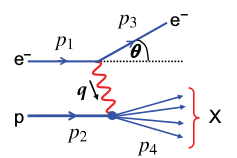
\includegraphics[width=0.3\textwidth]{subatom-02-kinematic.png}
\centering
\caption{Znázornenie kinematiky rozptylu.}
\label{sf2:fig:kinematics}
\end{figure}

Skúmanie štruktúry nukleónu pomocou rozptylu elektrónu. V závislosti na vlnovej dĺžke virtuálneho fotónu môžme rozlíšiť následujúce typy rozptylu elektrónu na nukleóne: 

\begin{figure}[!h]
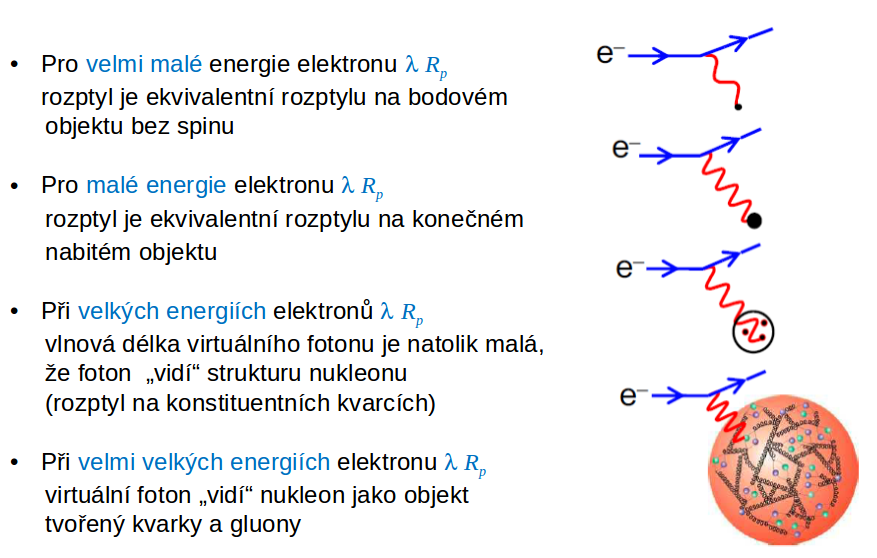
\includegraphics[width=1.0\textwidth]{subatom-02-typy.png}
\centering
\caption{Typy rozptylu.}
\label{sf2:fig:typy}
\end{figure}

Začneme elastickým rozptylom elektrónu na bodovom náboji. Pre tento typ rozptylu sme schopný odvodiť nasledujúci účinný prierez
\begin{equation}
 \frac{d\sigma}{dy} = \frac{2\pi \alpha^2}{Q^4}2p_1p_2 \left[ 1+(1-y)^2-\frac{M^2y}{p_1p_2} \right].
\end{equation}
V laboratórnej sústave má tento účinný prierez nasledujúci tvar
\begin{equation}
\frac{d\sigma}{d\Omega_{lab}} = \frac{\alpha^2 \cos^2(\theta/2)}{4E^2\sin^4(\theta/2)} \frac{E_3}{E_1} \bigg[ 1+\frac{Q^2}{2M^2\tan^2(\theta/2)} \bigg].
\end{equation}
V tejto poslednej formule sa prvý zlomok nazýva Mottov účinný prierez, ktorý je relativistické zovšeobecnenie pre Rutherfordov účinný prierez pre elastický rozptyl na Coulombovskom potenciály. Druhý zlomok je spôsobený spätným rázom protónu. Ako môžme vidieť pre elasticky rozptyl nám účinne prierezy závisia len na jednej premennej.

Keď budeme zvyšovať hodnotu $q$ tak sa elektrónu už nebude protón javiť ako bodová častica ale ako častica s nabitým konečným objemom. V takomto prípade už budeme musieť uvažovať rozloženie náboja v konečnom objeme. Toto rozloženie sa ošetrí použitím nasledujúceho potenciálu
$$ V({\vec{r}}) =\int \frac{Q\rho(\vec{r})}{4\pi \vert \vec{r}-\vec{r}^{\prime} \vert} d\vec{r}^{\prime} \hspace{1cm} kde \hspace{1cm} \int \rho(\vec{r})d\vec{r}=1 .$$
Berúc do úvahy takýto potenciál dostávame nasledujúci účinný prierez
\begin{equation}
\frac{d\sigma}{d\Omega_{lab}} = \frac{\alpha^2 \cos^2(\theta/2)}{4E^2 \sin^4(\theta/2)}\vert F(\vec{q}) \vert^2  \hspace{1cm} kde \hspace{1cm} F(\vec{q}) = \int \rho(\vec{r}^{\prime}) e^{i\vec{q}\vec{r}^{\prime}}d\vec{r}^{\prime}.
\label{sf2:mott}
\end{equation} 
Funkcia $F(\vec{q})$ sa nazýva formfaktor a má v sebe zakódovanú informáciu o štruktúre protónu. Napríklad pre bodový náboj má tento formfaktor hodnotu 1.
Na základe pozorovaní z experimentov sa daný účinný prierez spoločne s formfaktorom dá vyjadriť nasledovne
$$ \frac{d\sigma}{d\Omega} = \frac{\alpha^2}{4E_1^2\sin^2(\theta/2)} \frac{E_3}{E_1} \bigg( \frac{G^2_E + \tau G_M^2}{1+\tau}\cos^2(\theta/2)+2\tau G_M^2\sin^2(\theta/2) \bigg) \hspace{1cm} kde \hspace{1cm} \tau = \frac{Q^2}{4M^2_p}. $$
Tento vzťah má názov Rosenbluthová formula a popisuje pružný rozptyl na nukleóne konečnej veľkosti. V tejto formule sme zaviedli dva formfaktory, elektrický a magnetický, ktoré sa dajú vyjadriť nasledovne
\begin{equation}
\begin{gathered}
G_E(q^2) \approx \int \rho(\vec{r})e^{i\vec{q}\vec{r}} d\vec{r} \rightarrow G_E(0)=1  \\ 
G_M(q^2) \approx \int \mu(\vec{r})e^{i\vec{q}\vec{r}} d\vec{r} \rightarrow G_M(0)=\mu_{p}=2.79,
\end{gathered}
\end{equation} 
kde $G_E$ je spojené s distribúciou náboja a $G_M$ je spojené s distribúciou magnetického momentu. To, že $G_M=2.79$ znamená, že protón nie je bodová častica. 

Uveďme si nejaké experimenty, ktoré zohrali pri objavovaní štruktúry nukleónov významnú rolu:
\begin{itemize}
\item 1953, Stanford, Mark III Linac, skupina Hofstadtera  - systematické využívanie elektrónov k štúdiu štruktúry jadier, prvé experimenty s elektrónmi do energie $150\,\unit{MeV}$ potvrdili konečný rozmer jadier a aj to, že ich hranica nie je ostrá
\item 1955, skupina Hofstadtera - začala študovať štruktúru protónu elastickým rozptylom elektrónu na protóne pre $E < 200\,\unit{MeV}$
\item Hofstadter bol prvý človek, ktorý navrhol interpretovať elektrón-protónový účinný prierez z elastického rozptylu pomocou Mottovho účinného prierezu spoločne s vnútorným rozdelením nábojovej hustoty, tj. použitie rovnice (\ref{sf2:mott})
\item zvýšenie energie Mark III Linac na $550\,\unit{MeV}$, čo umožnilo zvýšiť presnosť merania až do $Q^2 \leq 0.5\,\unit{GeV^2}$
\item Mark III Linac s $1000\,\unit{MeV}$ zväzkom elektrónov - zo štúdií závislosti protónových formfaktoroch na $Q^2$ sa ukázalo, že magnetický a elektrický formfaktor sú si rovné v rámci chýb
\item 1962 - SLAC, elektróny s energiami do $20\,\unit{GeV}$ na štúdium elastických rozptylov elektrónu na protóne a iné
\item elastický rozptyl pri veľkom $Q^2 \rightarrow$ meranie $G_M(q^2)$, potvrdenie, že protón nie je bodová častica 
\end{itemize}

Po dosiahnutí dostatočne veľkých zrážkových energií bolo možné začať skúmať neelastické rozptyly. V tomto prípade nám už účinne prierezy budú závisieť na dvoch premenných. Dá sa ukázať, že najvšeobecnejšie vyjadrenie účinného prierezu pre neelastický rozptyl elektrónu na protóne má tvar
\begin{equation}
\frac{d\sigma}{dxdQ^2} = \frac{4\pi\alpha^2}{Q^2} \bigg[\bigg( 1-y-\frac{M^2y^2}{Q^2}\bigg)\frac{F_2(x,Q^2)}{x} +y^2F_1(x,Q^2) \bigg],
\label{sf2:blalbla}
\end{equation}
kde $F_1(x,Q^2)$ a $F_2(x,Q^2)$ sú magnetické a elektrické štruktúrne funkcie závislé na $x$ a $Q^2$ a nemôžu byť interpretované ako Fourierovské transformácie distribúcie náboja a magnetického momentu, tak ako to bolo v elastickom prípade. V skutočnosti popisujú hybnostnú distribúciu kvarkov v protóne.

Nato aby sme tieto funkcie určili pre dané $x$ a $Q^2$ by sme museli zmerať účinné prierezy v niekoľkých rozličných rozptylových uhloch a beam energiách. Experimentálne sa ukazuje, že tieto funkcie sú takmer nezávislé na $Q^2$. Táto skutočnosť je známa ako Bjorkenovo škálovanie:
$$ F_1(x,Q^2) \rightarrow F_1(x) \hspace{1cm} F_2(x,Q^2) \rightarrow F_1(x) $$

Takéto správania interpretujeme, že sa jedna o rozptyl elektrónu na bodových konštituentoch protónu\footnote{Usudzujeme z faktu, že pre elastický rozptyl nám magnetické a elektrické formfaktory, ktoré popisovali štruktúru protónu, záviseli na $Q^2$ z čoho sme následne vyvodili, že protón nie je bodová častica. Teraz nám ale štruktúrne funkcie skoro vôbec nezávisia na $Q^2$, čiže častice na ktorých sa elektrón rozptyľuje majú bodový charakter.}. Taktiež sa pozoruje, že $F_1(x)$ a $F_2(x)$ nie sú nezávislé ale platí pre ne tzv. Callan-Gross relácia
$$ F_2(x) = 2xF_1(x).$$
Táto relácia odráža fakt, že nabité zložky protónu nesú spin 1/2 a platí jedine vtedy, keď kvarky budú mať spin 1/2.

Uveďme teraz nejaké experimenty pre neelastické rozptyly
\begin{itemize}
\item 1968, Viedeň, konferencia ICHEP - riaditeľ SLAC-u prezentuje výsledky z neelastických experimentov, tieto výsledky naznačujú, že v nukleónoch sú nejaké štruktúry, ktoré majú bodový charakter
\item 1966-1978 SLAC-MIT kolaborácia, štúdium rozptylov vysoko-energetických elektrónov na protónoch a neutrónoch - experimenty, ktoré objavili malé objekty v protónoch a neutrónoch = kvarky
\end{itemize}

\subsection{Partónový model}
Predtým ako boli kvarky a gluóny akceptované, Feynman navrhol, že protón je zložený z bodových konštituentov, ktoré nazval partóny. Bjorkenovo škálovanie a Callan-Grossová relácia môžu byť vysvetlené predpokladajúc hlboký neelastický rozptyl virtuálneho fotónu na bodovej častici protónu so spinom 1/2. Partónový model sa ľahko formuluje v sústave, kde protón má veľkú energiu - INFINITE MOMENTUM FRAME, kde môžme zanedbať hmotnosť protónu a $p_2=(E_2,0,0,E_2)$. V tejto sústave taktiež môžme zanedbať hmotnosť kvarkov a akékoľvek predanie hybnosti do smeru protónu.

Nech kvark nesie čast $\xi$ z protónovej 4-hybnosti. Po interakcii má rozptýlený kvark hybnosť $\xi p_2+q$, potom môžme písať
$$ (\xi p_2+q)^2=m^2_q \approx 0 \rightarrow q^2+2p_2q=0 \hspace{1cm} kde \hspace{1cm} \xi^2 p_2^2 = m^2_q \approx 0, $$
potom dostávame $$ \xi = \frac{Q^2}{2p_2q} = x, $$
takže Bjorkenovo $x$ môže byť definovane ako časť protónovej hybnosti, ktorú nesie rozptýlený kvark, viď obrázok \ref{sf2:fig:parton}.

\begin{figure}[!h]
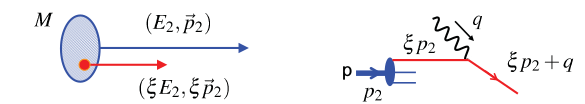
\includegraphics[width=0.8\textwidth]{subatom-02-parton.png}
\centering
\caption{Kinematika partónového modelu.}
\label{sf2:fig:parton}
\end{figure}

V konečnom dôsledku pre protón platí
$$ s=(p_1+p_2)^2\approx 2p_1p_2, \hspace{1cm} y=\frac{p_2q}{p_2 p_1}, \hspace{1cm} x=\frac{Q^2}{2p_2q},$$
a pre partón platí
$$ s_q=(p_+\xi p_2)^2=2xp_1p_2=xs, \hspace{1cm} y_q=\frac{p_qq}{p_qp_1}=\frac{xp_2q}{xp_2p_1} = y, \hspace{1cm} x_q=1 .$$
Skutočnosť, že $x_q=1$ nám napovedá, že sa jedná o elastický rozptyl, kvark sa neskladá už z ničoho. Pre účinný prierez dostávame 

\begin{equation}
\frac{d\sigma}{dQ^2} = \frac{4\pi\alpha^2 e_q^2}{Q^4}\bigg[ (1-y)+\frac{y^2}{2} \bigg]
\label{sf2:cross}
\end{equation}

Rovnica (\ref{sf2:cross}) je výraz pre diferenciálny účinný prierez pre elastický elektrón-kvark rozptyl, kde kvark nesie čast $x$ z protónovej hybnosti. Ďalej je potrebné zobrať do úvahy distribúciu hybnosti kvarku vo vnútri protónu. Zavádzame partónovú distribučnú funkciu tak, aby $q^p(x)dx$ opisovalo počet partónov typu $q$ vo vnútri protónu s frakciou hybnosti medzi $x$ a $x+dx$. Potom účinný prierez pre určitý typ kvarku nachádzajúci sa vo vnútri protónu, ktorý je v rozsahu $\left\langle x ; x+dx\right\rangle $ je

\begin{equation}
\frac{d\sigma}{dQ^2} = \frac{4\pi\alpha^2}{Q^4}\bigg[ (1-y)+\frac{y^2}{2} \bigg]\cdot e^2_q q^p(x)dx
\label{sf2:cross1}
\end{equation}

Presumovaním cez všetky kvarky dostávame

\begin{equation}
\frac{d\sigma}{dxdQ^2} = \frac{4\pi\alpha^2}{Q^4}\bigg[ (1-y)+\frac{y^2}{2} \bigg]\cdot \sum_q e^2_q q^p(x)
\label{sf2:cross2}
\end{equation}

Porovnaním rovnice (\ref{sf2:cross2}) a (\ref{sf2:blalbla}), kde zanedbáme hmotnostné členy, dostávame
$$ F_2(x,Q^2)=2xF_1(x,Q^2)=x\sum_q e^2_qg^p(x) $$
Z tejto rovnice pekne vidíme, že závislosť na $Q^2$ nie je badateľná (Bjorkenovo škálovanie) a taktiež vidíme ako sú tieto funkcie previazané (Callan-Gross relácia). Takže v konečnom dôsledku môžeme písať

\begin{figure}[!h]
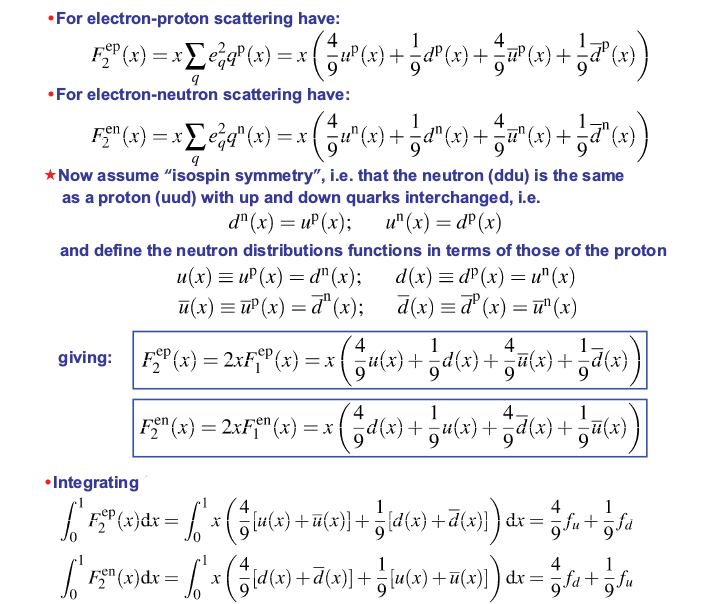
\includegraphics[width=1.0\textwidth]{subatom-02-pravidla.png}
\centering
\end{figure}

Z experimentov vychádza, že $f_u=0.36$ a $f_d=0.18$. Spolu to je 0.54, takže kvarky v protóne nesú len $50\%$ hybnosti, zvyšok nesú gluóny.

Partónové distribučné funkcie zahrňujú príspevky od valenčných kvarkov ale aj od virtuálnych kvarkov, ktoré sú produkované gluónmi tzv. morské kvarky.
Takže platí
$$ u(x) = u_v(x)+u_s(x) \hspace{1cm} d(x) = d_v(x)+d_s(x) $$
$$ \bar{u}(x) = \bar{u}_s(x) \hspace{1cm} \bar{d}(x) = \bar{d}_s(x),$$

kde pre protón dostávame
$$ \int_0^1u_v(x)dx=2 \hspace{1cm} \int_0^1d_v(x)dx=1 $$
 
Neočakáva sa žiadne množstvo pre celkový počet morských kvarkov. Morské kvarky pochádzajú z gluónov (vznik kvark-antikvark pár) a je rozumné očakávať $S(x)=u_s(x)=d_s(x)=\bar{u}_s(x)=\bar{d}_s(x)$. Potom 

\begin{figure}[!h]
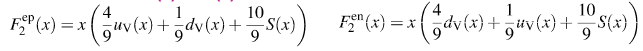
\includegraphics[width=0.9\textwidth]{subatom-02-rovnica.png}
\centering
\end{figure}

pomerom týchto členov dostávame nasledovné
$$ \frac{F^{en}_2(x)}{F^{ep}_2(x)}\rightarrow 1 \hspace{0.5cm} pre \hspace{0.5cm} x\rightarrow 0 $$
$$ \frac{F^{en}_2(x)}{F^{ep}_2(x)}\rightarrow \frac{4d_v(x)+u_v(x)}{4u_v(x)+d_v(x)} \rightarrow \frac{2}{3} \hspace{0.5cm} pre \hspace{0.5cm} x\rightarrow 1 \hspace{0.5cm} u_v(x)=2d_v(x) $$
Pre prvý zlomok je očakávané, že bude prevládať tvorba morských častíc takže očakávame, že ten zlomok rovný 1 (experimentálne potvrdené). Avšak, pre druhý zlomok sú očakávané 2/3 ale experimentálna hodnota je 1/4, čo je zatiaľ nevysvetlené.

\subsection{Jety}
Uvažujme kvark-antikvark pár produkovaný v elektrón-pozitrónovej anihilácii:
\begin{enumerate}
\item pôvodné kvarky sa začnú oddeľovať pri vysokej rýchlosti
\item sila, ktorá drží kvarky pohromade začne narastať 
\item energia uložená vo väzbe dosiahne také hodnoty, že je možné vytvoriť ďalší kvark-antikvark pár
\item tento proces pokračuje, až kým kvarky nevytvoria jety bezfarebných hadrónov
\end{enumerate}
Tento proces sa nazýva hadronizácia a zatiaľ nie je úplne matematicky popísaný. Hlavný dôsledok ale je, že v experimentoch kvarky a gluóny pozorujeme vo forme jetov častíc, viď obrázok \ref{sf2:fig:jet}.

\begin{figure}[!h]
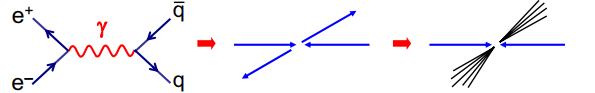
\includegraphics[width=0.8\textwidth]{subatom-02-jet.png}
\centering
\caption{Znázornenie produkcie jetu.}
\label{sf2:fig:jet}
\end{figure}

Zrážky $e^+e^-$ sú veľmi dobre pre štúdium QCD. Pretože QED je dobre popísaná, nepotrebujeme vedieť žiadne štruktúrne funkcie elektrónov pretože sa experimentálne jedná o čistý proces - neostávajú nám žiadne zvyšky z protónu alebo inej častice.
V týchto zrážkach je možné produkovať všetky typy kvarkov, treba nato však potrebnú energiu ($\sqrt{s}>2m_q$). Vo všeobecnosti, ak sa nevytvori viazaný stav kvarkov tak sa vytvorí jet hadrónov. Nevieme však povedať, ktorý jet pochádza z kvarku a ktorý z antikvarku. 

Využijeme klasický elektromagnetický proces ($e^+e^- \rightarrow \mu^+ \mu^-$).  Pre tento proces poznáme účinný prierez 
$$ \sigma = \frac{4\pi \alpha^2}{3s} \rightarrow \frac{d\sigma}{d\Omega} = \frac{\alpha^2}{4s}(1+\cos^2(\theta)).$$

Pre proces $e^+e^- \rightarrow q \bar{q}$ máme účinný prierez vo forme
$$ \sigma = 3 \sum_q \frac{4\pi \alpha^2}{3s} Q^2_q,$$ 
kde koeficient 3 je umelo vložený a je to dôsledok farebného náboja. Zvyčajne sa pozoruje pomer medzi týmito procesmi 
$$ \frac{\sigma(e^+e^- \rightarrow q\bar{q})}{\sigma(e^+e^- \rightarrow \mu^-\mu^+)} = 3 \sum_q Q^2_q.$$
Takže vidíme, že tento pomer nám závisí na počte a druhu kvarkov. Máme napríklad:
\begin{itemize}
\item pre u,d,s kvarky mame R=2
\item pre u,d,s,c kvarky mame R=10/3
\item pre u,d,s,c,b kvarky mame R=11/3
\end{itemize}

$e^+e^-$ zrážky sú dobré aj na štúdium gluónov, ktoré taktiež môžu vytvoriť jet. 

\begin{figure}[!h]
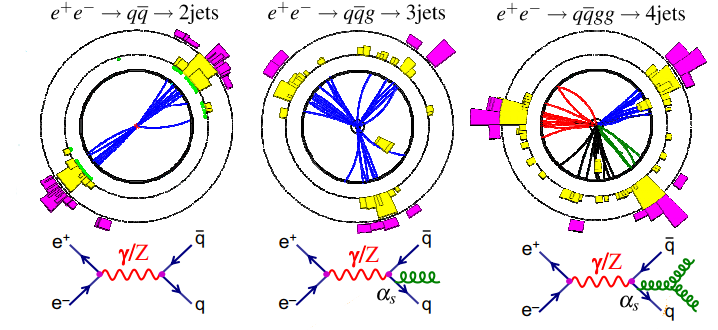
\includegraphics[width=0.8\textwidth]{subatom-02-gluon.png}
\centering
\caption{2 jety, 3 jety a 4 jety.}
\label{sf2:fig:gluon}
\end{figure}

\end{document}